\documentclass[9pt]{beamer}

% Videos
% V1, S 1-7
% V2, S 8-18
% V3, S 18-25
% V4, S 25-37

\setbeamersize{text margin left=6mm,text margin right=8mm}

\usetheme[progressbar=frametitle]{metropolis}

\usepackage{xcolor}



\definecolor{bluegreen}{RGB}{3, 166, 155}
\definecolor{pitchblack}{RGB}{0, 0, 0}
\definecolor{lightbeige}{RGB}{255, 251, 241}
\definecolor{mediumgray}{RGB}{183, 183, 183}
\definecolor{mygreen}{rgb}{0,0.6,0}
\definecolor{mygray}{rgb}{0.5,0.5,0.5}
\definecolor{mymauve}{rgb}{0.58,0,0.82}
\definecolor{keywords}{RGB}{255,0,90}
\definecolor{comments}{RGB}{0,0,113}
\definecolor{red}{RGB}{160,0,0}
\definecolor{green}{RGB}{0,150,0}
\definecolor{navy}{RGB}{0,0,128}




% \setbeamercolor{progress bar}{fg=green,bg=blue}
% \setbeamercolor{background canvas}{bg=pitchblack}
% \setbeamercolor{normal text}{fg=lightbeige}
% \setbeamercolor{frametitle}{bg=bluegreen, fg=mediumgray}
\setbeamercolor{background canvas}{bg=white}
\setbeamercolor{normal text}{fg=black}
\setbeamercolor{frametitle}{bg=white, fg=black}



\usepackage{appendixnumberbeamer}
\usepackage{booktabs}
\usepackage[scale=2]{ccicons}

\usepackage{pgfplots}
\usepgfplotslibrary{dateplot}

\usepackage{xspace}
\newcommand{\themename}{\textbf{\textsc{metropolis}}\xspace}

\usepackage{fancyhdr}
\usepackage[mmddyyyy,hhmmss]{datetime}

% \date{\today}
\date{}
% \date[Last Compiled:]{\today}

\author{Sambasiva Rao Gangineni, Harshad Reddy Nalla, Saeed Fathollahzadeh\\ and Kia Teymourian}
\institute{13th ACM International Conference on Distributed and Event-Based Systems - DEBS 2019}

% compiled: \today , Time: \currenttime}



% This is important to set the default font to serif.
\usefonttheme{serif} % default family is serif

% \setmainfont{Liberation Serif}

% Packages for drawing arrows.
\usepackage{tikz}
\usepgflibrary{arrows}% for more options on arrows

\usepackage{pgfplots}
\usepgfplotslibrary{dateplot}
\usepackage{xspace}
% \newcommand{\themename}{\textbf{\textsc{metropolis}}\xspace}

\usepackage{blindtext}

\usepackage{listings}

% \usepackage{color}

\usepackage{caption}
\usepackage{graphicx}



\definecolor{backgroundCol}{rgb}{.97, .97, .97}
\definecolor{commentstyleCol}{rgb}{0, 0, 80}
\definecolor{keywordstyleCol}{rgb}{0.737,0.353,0.396}
\definecolor{stringstyleCol}{rgb}{0.192,0.494,0.8}
\definecolor{NumCol}{rgb}{0.686,0.059,0.569}
\definecolor{basicstyleCol}{rgb}{0.345, 0.345, 0.345}



\lstset{ %
  language=R,                     % the language of the code
  basicstyle=\footnotesize  \ttfamily \color{basicstyleCol},       % the size of the fonts that are used for the code
  % numbers=left,                   % where to put the line-numbers
  % numberstyle=\tiny\color{gray},  % the style that is used for the line-numbers
  stepnumber=1,                   % the step between two line-numbers. If it's 1, each line
                                  % will be numbered
  numbersep=2pt,                  % how far the line-numbers are from the code
  backgroundcolor=\color{white},  % choose the background color. You must add \usepackage{color}
  showspaces=false,               % show spaces adding particular underscores
  showstringspaces=false,         % underline spaces within strings
  showtabs=false,                 % show tabs within strings adding particular underscores
  frame=single,                   % adds a frame around the code
  rulecolor=\color{black},        % if not set, the frame-color may be changed on line-breaks within not-black text (e.g. commens (green here))
  tabsize=1,                      % sets default tabsize to 2 spaces
  captionpos=b,                   % sets the caption-position to bottom
  breaklines=true,                % sets automatic line breaking
  breakatwhitespace=false,        % sets if automatic breaks should only happen at whitespace
  title=\lstname,                 % show the filename of files included with \lstinputlisting;
                                  % also try caption instead of title
  keywordstyle=\color{keywordstyleCol},      % keyword style
  commentstyle=\color{commentstyleCol},   % comment style
  stringstyle=\color{stringstyleCol},      % string literal style
  escapeinside={\%*}{*)},         % if you want to add a comment within your code
  morekeywords={*,...},            % if you want to add more keywords to the set
  belowskip=-0.8 \baselineskip
}


\usepackage{algpseudocode}
\usepackage{MnSymbol,wasysym}

\definecolor{DarkGrenen}{RGB}{0,100,0}
\definecolor{DarkOliveGreen}{RGB}{85,107,47}

\definecolor{saddlebrown}{RGB}{139,69,19}




\newcommand{\red}[1]{\textcolor{red}{#1}}
\newcommand{\blue}[1]{\textcolor{blue}{#1}}
\newcommand{\green}[1]{\textcolor{DarkGrenen}{#1}}
\newcommand{\brown}[1]{\textcolor{saddlebrown}{#1}}


\newcommand{\redb}[1]{\textcolor{red}{\textbf{\boldmath{#1}}}}
\newcommand{\blueb}[1]{\textcolor{blue}{\textbf{\boldmath{#1}}}}
\newcommand{\greenb}[1]{\textcolor{DarkGrenen}{\textbf{\boldmath{#1}}}}
\newcommand{\brownb}[1]{\textcolor{saddlebrown}{\textbf{\boldmath{#1}}}}

\usepackage{url}


\usepackage{wrapfig}

\usepackage{subcaption}


% \usepackage[parfill]{parskip}



\title[Real-Time Object Recognition from Streaming LiDAR Point Cloud Data]{Grand Challenge: Real-Time Object Recognition 
from Streaming LiDAR Point Cloud Data}



\begin{document}

\setbeamertemplate{itemize item}{\color{red}$\triangleright$}
\setbeamertemplate{itemize subitem}{\color{blue}$\triangleright$}
% \setbeamertemplate{footline}[page number]{}

% \defbeamertemplate*{footline}{infolines theme}
% {
%   \leavevmode%
%   \hbox{%
%   \begin{beamercolorbox}[wd=1\paperwidth,ht=0.1ex,dp=3.5ex,right]{date in
%   head/foot}%
%     	\usebeamerfont{date in head/foot}\insertshortdate{}\hspace*{2em}
% 		\insertframenumber{} / \inserttotalframenumber\hspace*{3ex}
%   \end{beamercolorbox}}%
%   \vskip0pt%
% }




\setbeamertemplate{navigation symbols}{}

% \setlist{nosep,after=\vspace{\baselineskip}}

\maketitle





%%%%%%%%%%%%%%%%%%%%%%%%%%%%%%%%%%%%%%%%%%%%
%%%%%%%%%%%%%%%%%%%%%%%%%%%%%%%%%%%%%%%%%%%%

\begin{frame}{Table of contents}
 \setbeamertemplate{section in toc}[sections numbered]
   \tableofcontents[hideallsubsections]


\end{frame}



%%%%%%%%%%%%%%%%%%%%%%%%%%%%%%%%%%%%%%%%%%%%%%%%%%%%%
%%%%% Challenges with the data %%%%%%
%%%%%%%%%%%%%%%%%%%%%%%%%%%%%%%%%%%%%%%%%%%%%%%%%%%%%

\begin{frame}[fragile]{Challanges with the data}
	\begin{itemize}
		\item Training data has input file and output file, input file has the coordinates and output has object names and the count of the each object.
		\item But there are no annotations.
		\item There are single-object scenes and multiple object scenes in the training data.
		\item Because of this problem, we cannot use the multiple-object scenes in the training phase. Also, this helped us to design our data processing pipeline.
	\end{itemize}
\end{frame}



%%%%%%%%%%%%%%%%%%%%%%%%%%%%%%%%%%%%%%%%%%%%
%%%%%%%%%%%%%%%%%%%%%%%%%%%%%%%%%%%%%%%%%%%%

\section{Data Processing Pipleline}


%%%%%%%%%%%%%%%%%%%%%%%%%%%%%%%%%%%%%%%%%%%%
%%%%%%%%%%%%%%%%%%%%%%%%%%%%%%%%%%%%%%%%%%%%

\begin{frame}[fragile]{Architecture}
\redb{Steps for data processing:}
\begin{itemize}
	\item \blueb{Step 1:} Data Filtering (Training and Testing)
	\item \blueb{Step 2:} Object Segmentation (Testing)
	\item \blueb{Step 3:} Object Classification (Training and Testing)
\end{itemize}

\begin{figure}
	\centering
	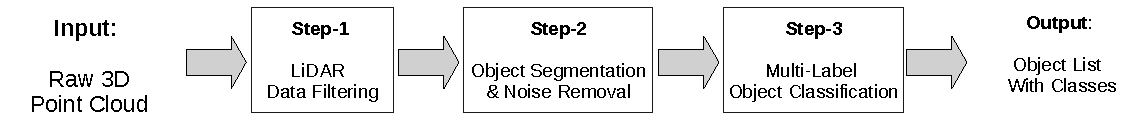
\includegraphics[width=\textwidth]{images/DataProcessingPipleline.pdf}

\end{figure}
\end{frame}


%%%%%%%%%%%%%%%%%%%%%%%%%%%%%%%%%%%%%%%%%%%%
%%%%%%%%%%%%%%%%%%%%%%%%%%%%%%%%%%%%%%%%%%%%

\begin{frame}[fragile]{Step 1: LiDAR Laser Line Data Filtering}
	\begin{itemize}
		\item Filter out the LiDAR laser lines that build
		a cylinder 3D shape from the laser standing point $(x=0, y=0, z=0)$.
		\item Figure 1 visualizes the LiDAR data for a single scene with LiDAR laser lines and Figure 2 visualizes the data after
		filtering out the Laser lines.
	\end{itemize}

	\begin{columns}
		\begin{column}{0.48\textwidth}
			\begin{figure}
				\centering
				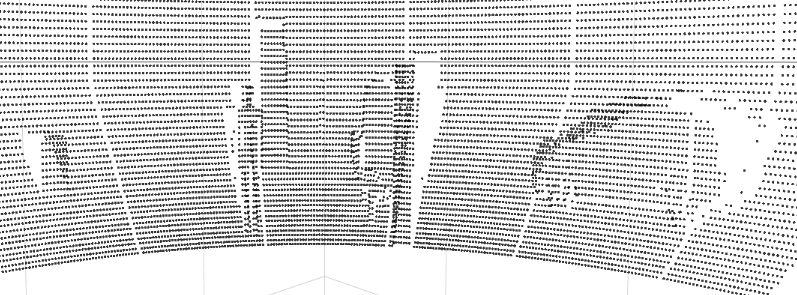
\includegraphics[width=\textwidth]{images/ground_before2.png}
				\caption{LiDAR Raw Point Cloud Data}
			\end{figure}
		\end{column}
		\begin{column}{0.48\textwidth}
			\begin{figure}
				\centering
				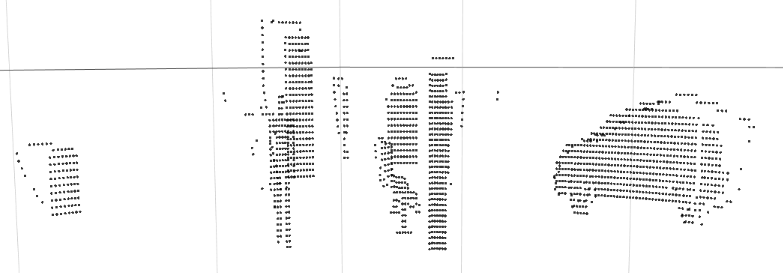
\includegraphics[width=\textwidth]{images/ground_after2.png}		\caption{Data After Filtering the LiDAR Scan Lines}
			\end{figure}
		\end{column}
	\end{columns}

\end{frame}

%%%%%%%%%%%%%%%%%%%%%%%%%%%%%%%%%%%%%%%%%%%%%%%%%%%%%%%%
%%%%% Algorithm for removing the ground points %%%%%%
%%%%%%%%%%%%%%%%%%%%%%%%%%%%%%%%%%%%%%%%%%%%%%%%%%%%%

\begin{frame}[fragile]{Step 1: Contd.}
	\redb{Understanding the 3D cylinder}
	\begin{itemize}
		\item In the given data each point is annotated with the laser number.
		\item LiDAR used for collecting this data is mounted with the 64 lasers, each with different angle of elevation. Each cylinder line is formed by a single laser.
		\item In an empty scene and flat ground, the distance of the points in each cylinder line from the LiDAR is always constant.
		\item Thus, all the boundary points for each laser will always correspond to same distance given that the vehicle used to mount LiDAR is same.
	\end{itemize}
\end{frame}

%%%%%%%%%%%%%%%%%%%%%%%%%%%%%%%%%%%%%%%%%%%%
%%%%%%%%%%%%%%%%%%%%%%%%%%%%%%%%%%%%%%%%%%%%

\begin{frame}[fragile]{Step 2: Object Segmentation and Noise Removal}
	\redb{segment the point cloud to chunks of data}
	\begin{itemize}
		\item \blueb{3D to 2D Projection:} projected the 3D data in 4 different ways to a 2D plane and reduced the data dimensionality

		\item \blueb{Perspective projection}:
		\begin{align*}
		d  & = \text{Distance to a projection plane} \\
		x' & =  x (\frac{d}{z}) \ \  , \ \  y' =  y (\frac{d}{z}) \ \  , \ \  z'=  z (\frac{d}{z}) = d
		\end{align*}

		\item Object points have varying density when the surface of the object is not normal to the LiDAR. To make the object points dense 2D projections are used.
	\end{itemize}
\end{frame}


%%%%%%%%%%%%%%%%%%%%%%%%%%%%%%%%%%%%%%%%%%%%
%%%%%%%%%%%%%%%%%%%%%%%%%%%%%%%%%%%%%%%%%%%%

\begin{frame}[fragile]{Step 2: Object Segmentation - Contd. }
	\redb{Distance based vs Density based Clustering}
	\begin{itemize}
		\item \blueb{Object segmentation using Clustering:} different clustering methods to cluster the data
		\begin{enumerate}
			\item \textbf{K-means and Mini Batch K-means} on the 3D and project 2D data.
			\item \textbf{Meanshift} on 3D and 2D data
			\item \textbf{DBSCAN} on 3D and 2D
		\end{enumerate}
		\item Figure 3 visualizes the data after filtering the LiDAR lines and Figure 4 visualizes the objects after clustering
	\end{itemize}

	\begin{columns}
		\begin{column}{0.48\textwidth}
			\begin{figure}
				\centering
				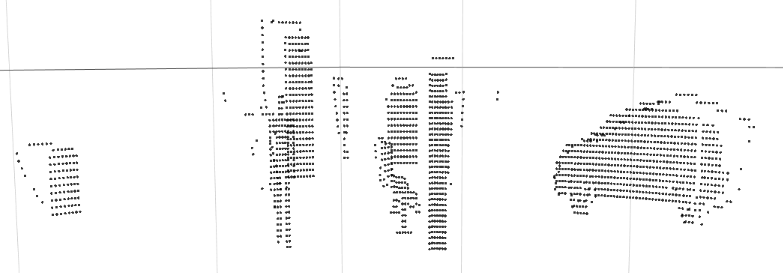
\includegraphics[width=\textwidth]{images/ground_after2.png}
				\caption{Data after Filtering the LiDAR Scan Lines}
			\end{figure}
		\end{column}
		\begin{column}{0.48\textwidth}
			\begin{figure}
				\centering
				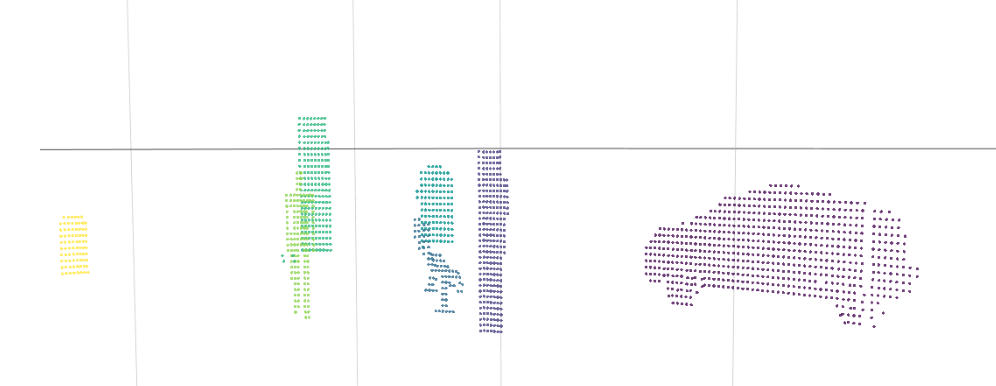
\includegraphics[width=\textwidth]{images/seg_noise_removal.png}		
				\caption{Clustered Point Cloud Data}
			\end{figure}
		\end{column}
	\end{columns}

\end{frame}




%%%%%%%%%%%%%%%%%%%%%%%%%%%%%%%%%%%%%%%%%%%%
%%%%%%%%%%%%%%%%%%%%%%%%%%%%%%%%%%%%%%%%%%%%

\begin{frame}[fragile]{Step 2: Object Segmentation - Top-View }

\redb{One 2D Projection Idea}

\begin{columns}
	\begin{column}{0.48\textwidth}
		\begin{figure}
			\centering
			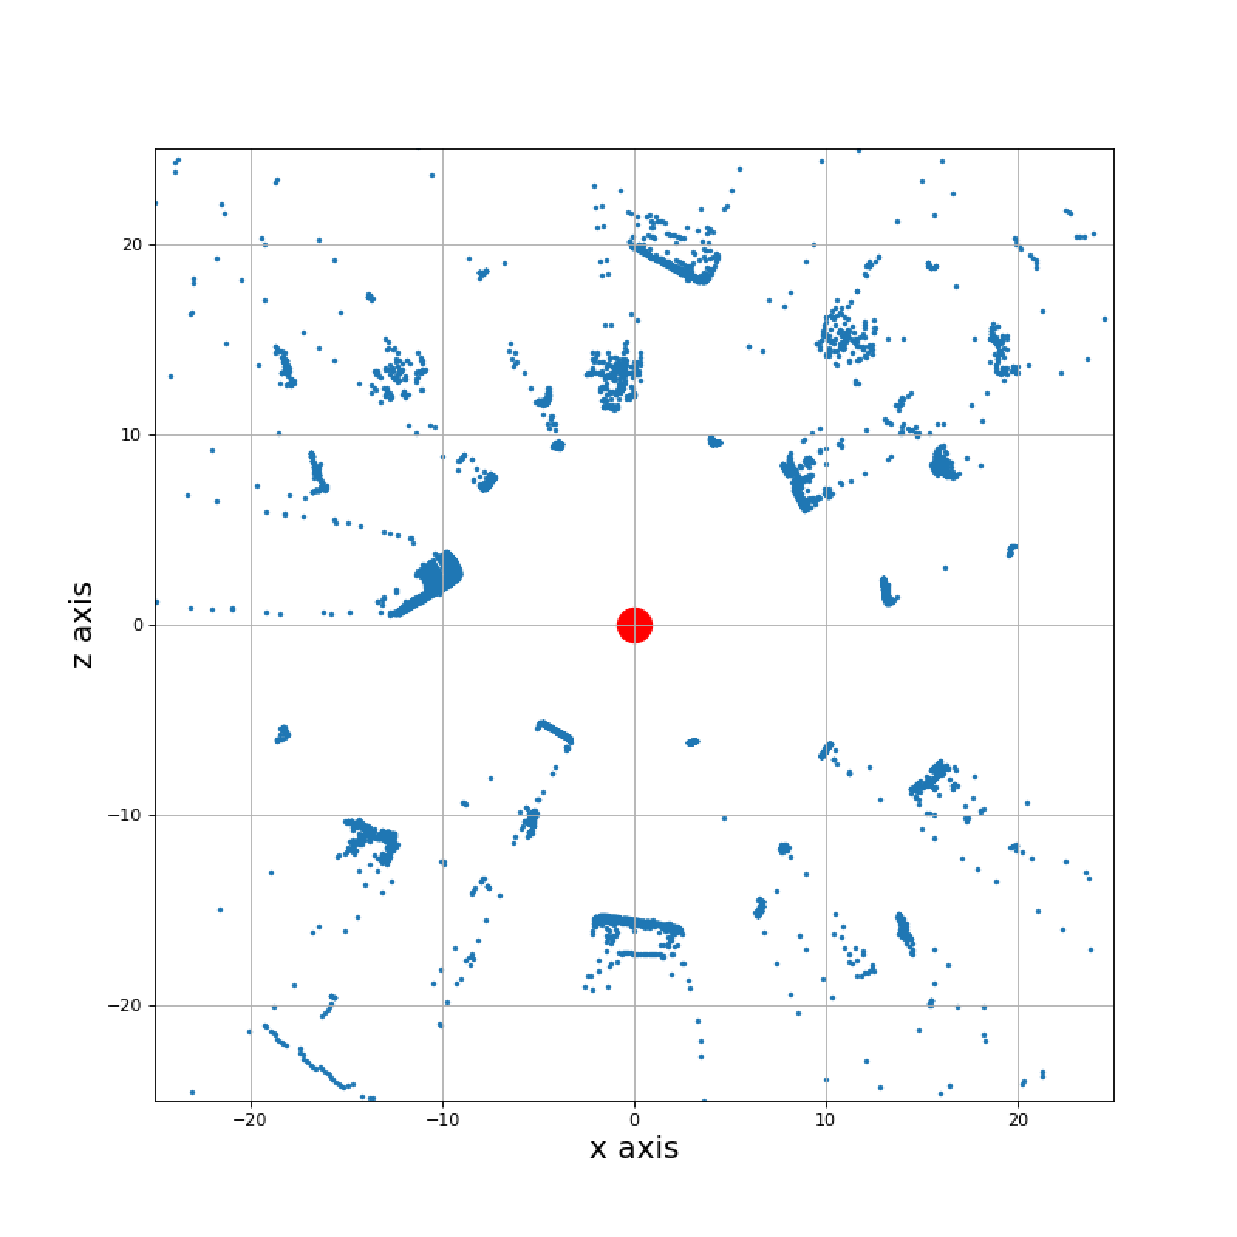
\includegraphics[width=\textwidth]{./images/sector-transforms/scene-with-centre.pdf}
			 \caption{Top-View of LiDAR Data}
		\end{figure}
	\end{column}
	\begin{column}{0.48\textwidth}
		\begin{figure}
			\centering
			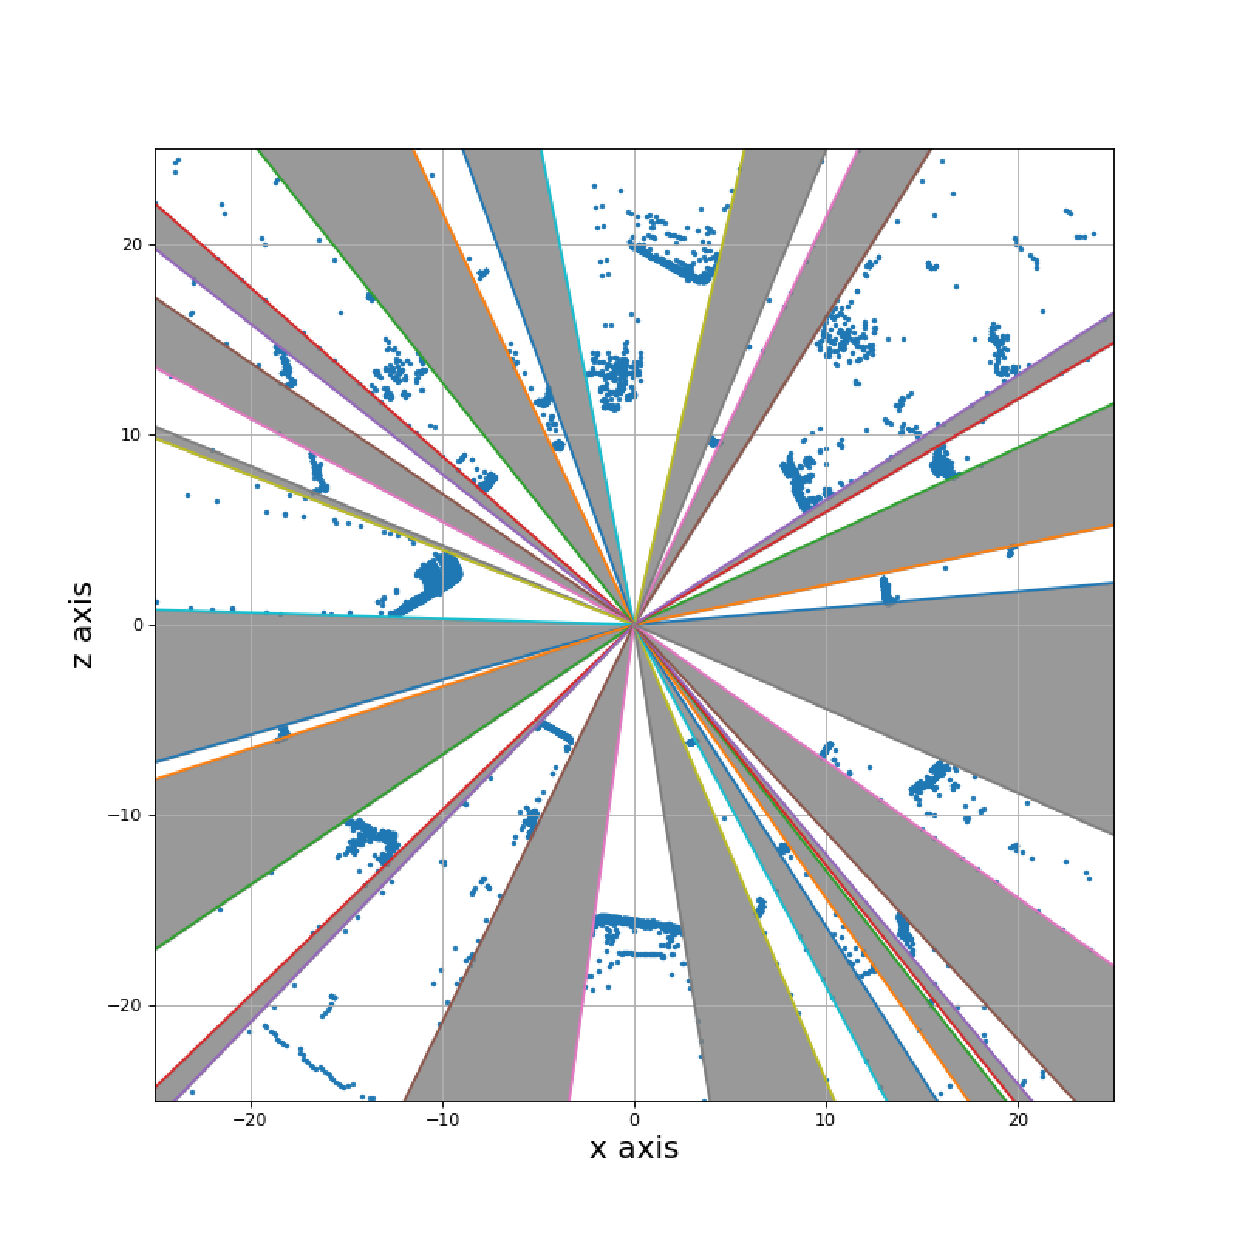
\includegraphics[width=\textwidth]{./images/sector-transforms/scene-with-sector.pdf}		
			\caption{Top-View - Separating unoccupied spaces/sectors (gray colored) from sectors with objects}
		\end{figure}
	\end{column}
\end{columns}

\end{frame}



%%%%%%%%%%%%%%%%%%%%%%%%%%%%%%%%%%%%%%%%%%%%%%%%%%%%%
%%%%% Proposed solution for the clustering %%%%%%
%%%%%%%%%%%%%%%%%%%%%%%%%%%%%%%%%%%%%%%%%%%%%%%%%%%%%


%%%%%%%%%%%%%%%%%%%%%%%%%%%%%%%%%%%%%%%%%%%%
%%%%%%%%%%%%%%%%%%%%%%%%%%%%%%%%%%%%%%%%%%%%

\begin{frame}[fragile]{Step 3: Multi-class Object Classification}
	Used for classification of point cloud data Convolutional Neural Network (CNN)

	\redb{Layers:}
	\begin{itemize}
		\item Convolutional layer
		\item Max Pooling layer
		\item Dropout Layer
		\item Fully Connected Layer
	\end{itemize}

	\begin{figure}
		\centering
		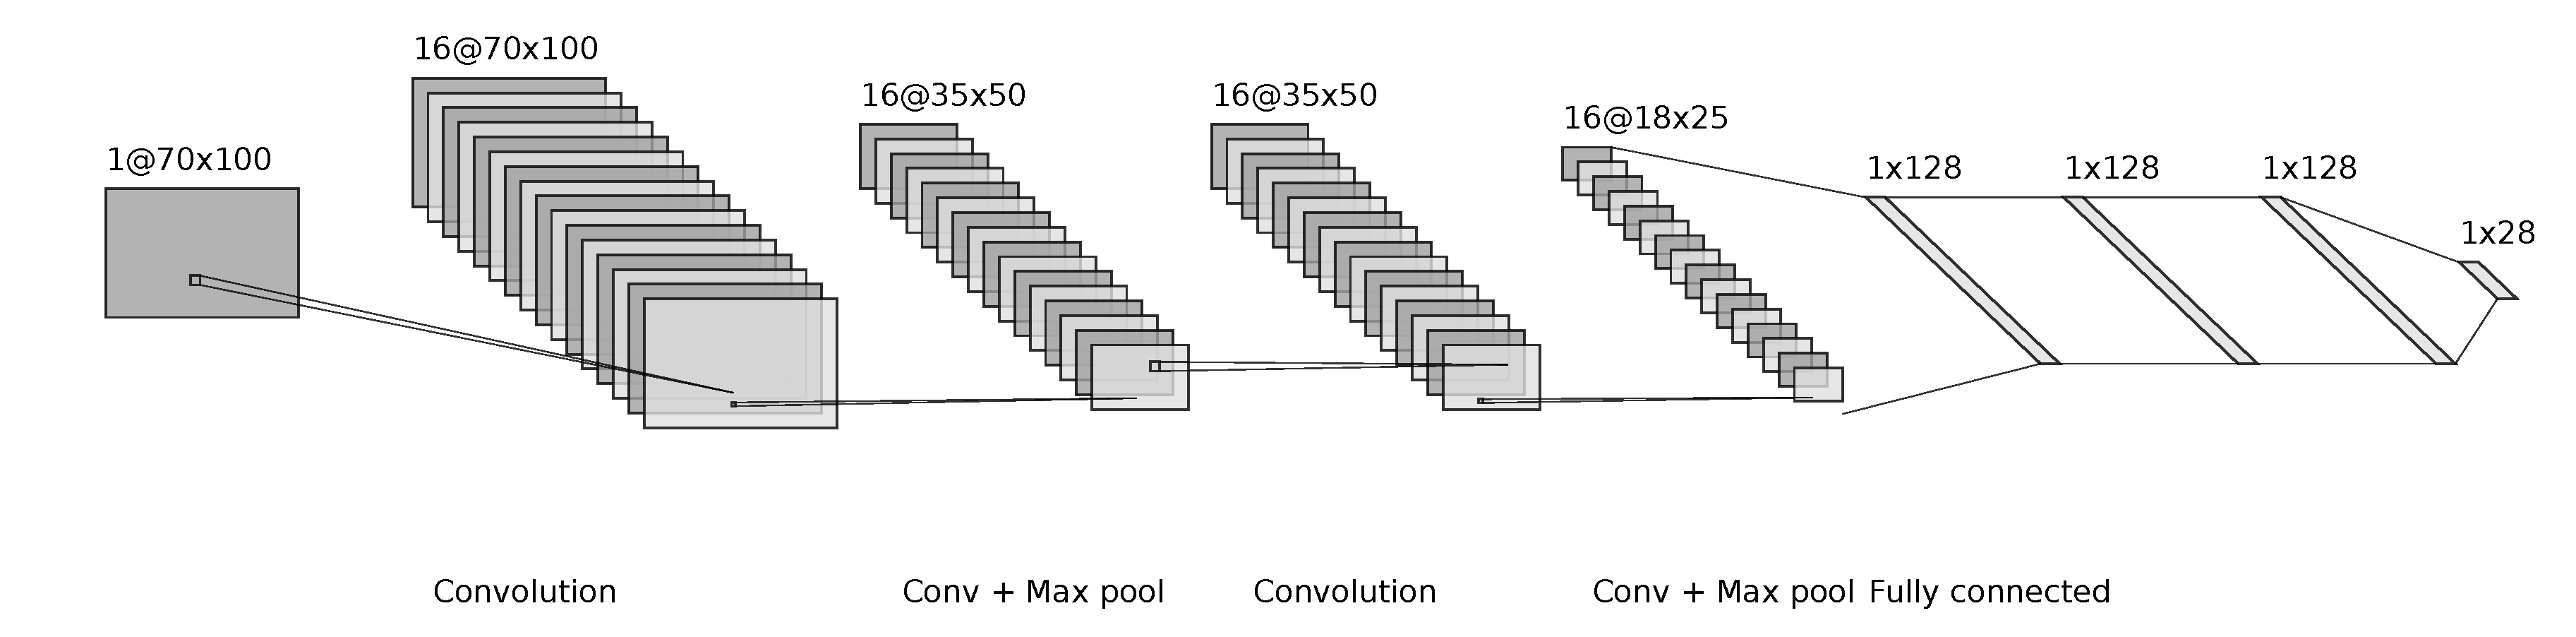
\includegraphics[width=\textwidth]{images/object_net.pdf}

	\end{figure}
\end{frame}

%%%%%%%%%%%%%%%%%%%%%%%%%%%%%%%%%%%%%%%%%%%%%%%%%%%%%
%%%%% Data Preparation for training %%%%%%
%%%%%%%%%%%%%%%%%%%%%%%%%%%%%%%%%%%%%%%%%%%%%%%%%%%%%

\begin{frame}[fragile]{Preparing Input data}
	\begin{itemize}
		\item The 3D points of the object are projected to 2D using one of the techniques.
		\item The projected points are placed in a grid of $7 \times 10$
		\item This grid is divided into cells of $0.1 \times 0.1$, resulting in $70 \times 100$ cells.
		\item The number of points in each cell is the input to the model.
		\item This input on plotting as pixels is as follows
	\end{itemize}

	\begin{columns}
		\begin{column}{0.33\textwidth}
			\begin{figure}
				\centering
				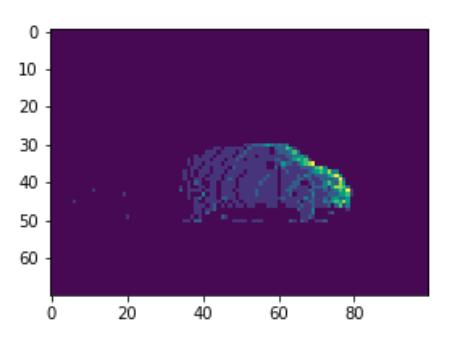
\includegraphics[width=\textwidth]{images/Toyota.png}
				\caption{Toyota}
			\end{figure}
		\end{column}
		\begin{column}{0.33\textwidth}
			\begin{figure}
				\centering
				\includegraphics[width=\textwidth]{images/Tractor.png}		
				\caption{Tractor}
			\end{figure}
		\end{column}
		\begin{column}{0.33\textwidth}
			\begin{figure}
				\centering
				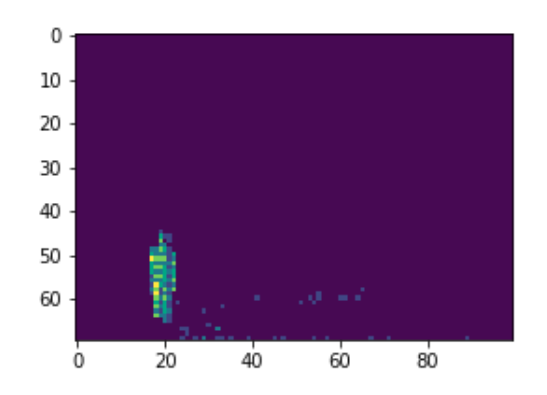
\includegraphics[width=\textwidth]{images/pedestrian.png}		
				\caption{Pedestrain}
			\end{figure}
		\end{column}
	\end{columns}

\end{frame}

%%%%%%%%%%%%%%%%%%%%%%%%%%%%%%%%%%%%%%%%%%%%
%%%%%%%%%%%%%%%%%%%%%%%%%%%%%%%%%%%%%%%%%%%%

\begin{frame}[fragile]{Training and Testing}
	\redb{Training: only single object scenes are used}
\begin{itemize}
	\item Using Step 1 filter the data
	\item Prepare the input for the model and train the model
\end{itemize}

\redb{Testing: Both single object and multiple object scenes can be used}

\begin{itemize}
	\item Using Step 1 filter the data
	\item Using Step 2 do the segmentation
	\item Prepare the input to the model and test the data
\end{itemize}

Note: Segmentation is done only in the testing.

\end{frame}




%%%%%%%%%%%%%%%%%%%%%%%%%%%%%%%%%%%%%%%%%%%%
%%%%%%%%%%%%%%%%%%%%%%%%%%%%%%%%%%%%%%%%%%%%

\section{Evaluation}

%%%%%%%%%%%%%%%%%%%%%%%%%%%%%%%%%%%%%%%%%%%%
%%%%%%%%%%%%%%%%%%%%%%%%%%%%%%%%%%%%%%%%%%%%

\begin{frame}[fragile]{Evaluation: Accuracy and Loss }
	\redb{Training and Validation Accuracy and Loss}
	\begin{figure}
		\centering
		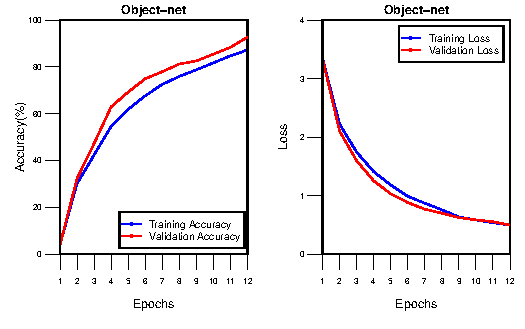
\includegraphics[width=\textwidth]{images/one_to_one.pdf}

	\end{figure}
\end{frame}

\begin{frame}[fragile]{Experiment Setups }
\redb{We evaluated our implementation \footnote{Github Repository
	of our Implementation \url{https://github.com/kiat/debs2019}} using the 4 different experiment setups:}
\begin{itemize}
	\item 2-Layer CNN on projected data to 2D (Single View) and Object Segmentation with 3D DBSCAN
	\item 2-Layer CNN on projected data to 2D (Using perspective projection) and Object Segmentation with 3D DBSCAN
	\item 4-Layer CNN on projected data to 2D (Single View) and Object Segmentation with 3D DBSCAN
	\item 4-Layer CNN on projected data to 2D (Using perspective projection) and Object Segmentation with 3D DBSCAN
\end{itemize}

\end{frame}


\begin{frame}[fragile]{Evaluation: Experiment Settings on DEBS2019 }
\redb{Precision, Recall, Accuracy and Processing Time of 4 different our Experiment Variation}
\begin{figure}
	\centering
	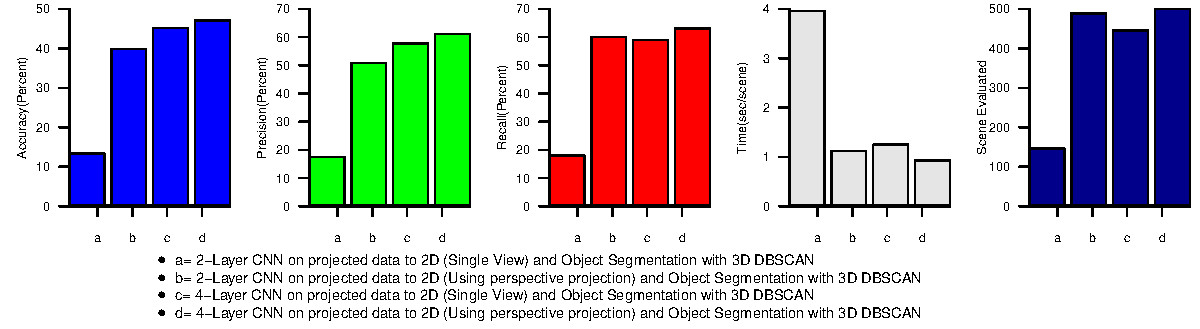
\includegraphics[width=\textwidth]{images/evaluation2.pdf}

\end{figure}
\end{frame}

%%%%%%%%%%%%%%%%%%%%%%%%%%%%%%%%%%%%%%%%%%%%
%%%%%%%%%%%%%%%%%%%%%%%%%%%%%%%%%%%%%%%%%%%%
\section{Related Work}
\begin{frame}[fragile]{Related Work}
	\redb{In this brief section, we review some of the most related publications regarding LiDAR point cloud object recognition problem.}

	\begin{itemize}
		\item  \cite{DBLP:journals/corr/abs-1811-01571}
		introduces multi-view stereographic projection; it first transforms a 3D input volume into a 2D planar image using stereographic projection.

		\item \cite{Zhou_2018_CVPR} is the best-ranked model on KITTI \cite{geiger2012we} for 3D and birds-eye view detections using LiDAR data only

		\item \cite{DBLP:conf/icra/WuWYK18} present SqueezeSeg which projects point cloud to the front view with cells gridded by LiDAR rotation

		\item \cite{DBLP:conf/cvpr/RieglerUG17} design more efficient 3D CNN or neural network architectures that exploit sparsity in the point cloud

		\item \cite{DBLP:conf/icpr/HuangY16} take a point cloud and parse it through a dense voxel grid, generating a set of occupancy voxels which are used as input to a 3D CNN to produce one label per voxel

		\item \cite{DBLP:conf/iros/MaturanaS15} used deep learning models is to first convert raw point cloud data into a
		volumetric representation, namely a 3D grid



	\end{itemize}
%\resizebox{\linewidth}{!}{
%	\begin{tabular}{*{3}{l}}
%		\toprule
%		Yavartanoo \cite{DBLP:journals/corr/abs-1811-01571}  & A & B\\
%		\midrule
%		One   & 1 & 2 \\
%		Two   & 26 & 25 \\
%		\bottomrule
%	\end{tabular}
%}

\end{frame}

%%%%%%%%%%%%%%%%%%%%%%%%%%%%%%%%%%%%%%%%%%%%
%%%%%%%%%%%%%%%%%%%%%%%%%%%%%%%%%%%%%%%%%%%%

\section{Conclusion}
\begin{frame}[fragile]{Conclusion }
\redb{Lessons learned from our implementation are}:
\begin{itemize}
	\item Classification of LiDAR point cloud can achieve high accuracy and real-time processing time by projecting the 3D data into 2D view.
	\item Classification using CNN on point cloud does not need a large number of hidden layers to achieve high accuracy.
	\item Segmentation may fail if the scene includes tiny objects or objects have variable density like ``Tree Objects''.
	\item If multiple objects are in a scene and they are hiding each other (completely or partially) then object segmentation using DBSCAN
	or other traditional clustering methods may fail to separate objects.
\end{itemize}
\end{frame}

%%%%%%%%%%%%%%%%%%%%%%%%%%%%%%%%%%%%%%%%%%%%
%%%%%%%%%%%%%%%%%%%%%%%%%%%%%%%%%%%%%%%%%%%%

\appendix
\begin{frame}[fragile]{}

\centering
\Huge
Thank you!

\end{frame}

%%%%%%%%%%%%%%%%%%%%%%%%%%%%%%%%%%%%%%%%%%%%
%%%%%%%%%%%%%%%%%%%%%%%%%%%%%%%%%%%%%%%%%%%%
\section{References}
\begin{frame}[allowframebreaks]{References}

	%	\bibliographystyle{apalike}
	\bibliographystyle{apalike}
	\bibliography{references}

\end{frame}


%%%%%%%%%%%%%%%%%%%%%%%%%%%%%%%%%%%%%%%%%%%%
%%%%%%%%%%%%%%%%%%%%%%%%%%%%%%%%%%%%%%%%%%%%

\appendix
\begin{frame}[fragile]{}

\centering
\Huge
Backup Slides

\end{frame}



%%%%%%%%%%%%%%%%%%%%%%%%%%%%%%%%%%%%%%%%%%%%
%%%%%%%%%%%%%%%%%%%%%%%%%%%%%%%%%%%%%%%%%%%%
\begin{frame}[fragile]{Real-time Data Stream Processing}
How to achieve real-time stream processing? 
	
\begin{itemize}
	\item \blueb{Step 1:} Data Filtering
	\item \blueb{Step 2:} Object Segmentation
	\item \blueb{Step 3:} Object Classification
\end{itemize}

Fast algorithm and efficient implementation. 

\begin{itemize}
	\item Choose appropiate alogirthm
	\item Be caution about all implementation details
\end{itemize}

\end{frame}

\end{document}
